
\begin{figure}[H]
  \begin{center}
      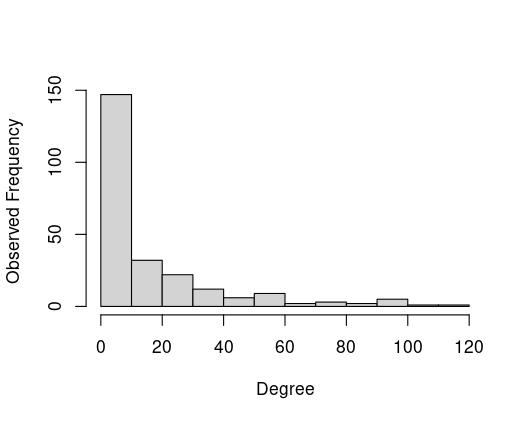
\includegraphics[width=\textwidth]{Fruglink/supplement/figs/FigS1.png}
    \caption[Observed degree distribution of avian frugivores]{Observed degree distribution of avian frugivore species included in our analyses. X-axis represents node degree, or number of unique partners. Degree for frugivores ranged from 1 (53 species) to 120 unique plant interactions recorded for \emph{Turdus rufiventris}; median frugivore degree was 5.}
    \label{fig:FruglinkS1}
  \end{center}
\end{figure}

\begin{figure}[H]
  \begin{center}
      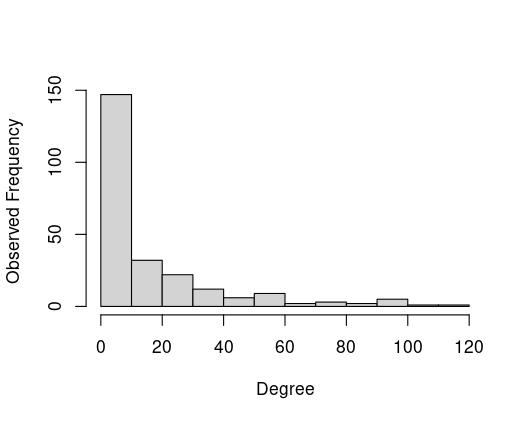
\includegraphics[width=\textwidth]{Fruglink/supplement/figs/FigS1.png}
    \caption[Observed degree distribution of avian plant species]{Observed degree distribution of plant species included in our analyses. X-axis represents node degree, or number of unique partners. Degree on average tended to be lower for plants than frugivores; plant node degree ranged from 1 (128 species) to 80 unique frugivorous interactions recorded for \emph{Myrsine coriacea}; median plant degree was 5.}
    \label{fig:FruglinkS2}
  \end{center}
\end{figure}

\begin{table}[ht]
\centering
\begin{tabular}{lrrr}
\hline
Model & Number of Links & Number of Bird species & Number of Plant spp \\
\hline
Latent & 3856 & 242 & 458 \\
Phy & 3276 & 225 & 377 \\
Traits & 2813 & 159 & 283 \\
PhyLatent & 3276 & 225 & 377 \\
PhyTraits & 2492 & 157 & 246 \\
TraitsLatent & 2813 & 159 & 283 \\
Trio & 2492 & 157 & 246 \\
\hline
\end{tabular}
\caption[Number of interactions, unique bird species, and unique plant species used in each model]{Number of interactions, unique bird species, and unique plant species used in each model. Incomplete modeling cases were dropped from each model; the remaining number of complete cases was shown below.}
\label{tab:model_summary}
\end{table}


\paragraph*{Impact of Phylogenetic Imputation}\mbox{}\\
In our main text results, for the 46 plant species and 2 bird species which did not appear in the appropriate phylogenies but did have congenerics, we randomly assigned those species to be a polytomy within their parent genera. When these species are excluded from the analysis, our results are still qualitatively indistinguishable. Below are versions of the three main-text figures with those 48 species removed from the network. 

\begin{figure}[H]
  \begin{center}
      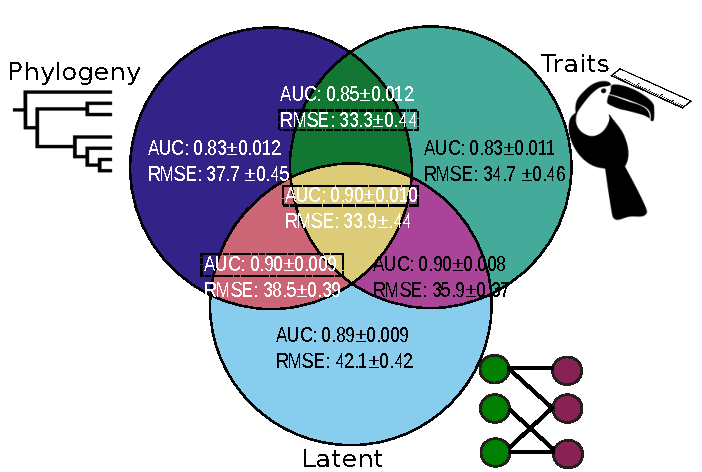
\includegraphics[width=\textwidth]{Fruglink/supplement/figs/ReplicatePerformance_CV_NoPolytomies.pdf}
    \caption[Summary performance metrics of all 7 models when species without full phylogenetic information are excluded]{Summary performance metrics of all 7 models *when species without full phylogenetic information are excluded*, as measured by area under the receiver operating characteristic curve (AUC) and root mean squared error (RMSE); highest performing models for each metric are outlined in dashed (AUC) or dotted lines (RMSE). Mean metric values are presented from 100 replicates of each model structure alongside standard deviation. As in the main text, model discriminatory power between links and non-links is maximized by including latent structural features, with the inclusion of trait, phylogenetic information, or both actually slightly decreasing discriminatory power. However, inclusion of trait and phylogenetic information, while not improving AUC, does increase overall model accuracy as measured by mean root squared error. Pairwise \emph{t}-test adjusted for multiple comparisons showed no significant difference between the discriminatory power of the highest performing models (Trio, PhyLatent, $p=0.24$)}
    \label{fig:FruglinkS3}
  \end{center}
\end{figure}

\begin{figure}[H]
  \begin{center}
      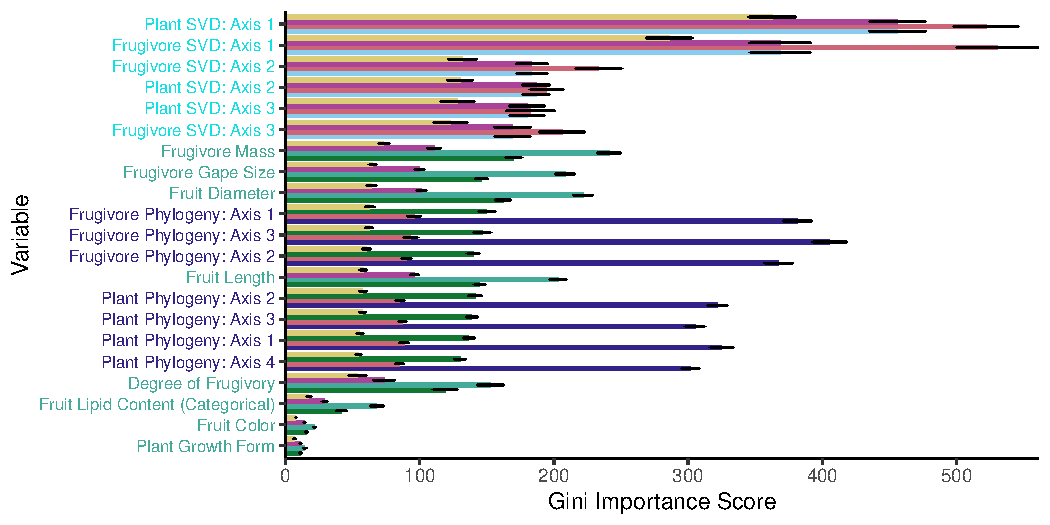
\includegraphics[width=\textwidth]{Fruglink/supplement/figs/VarImportance_ErrBars_Short_col2_withCV_noPoly.pdf}
    \caption[Variable importance across all models as measure by Gini importance score when species without full phylogenetic information are excluded]{Variable importance across all models as measure by Gini importance score *when species without full phylogenetic information are excluded*; color scheme is consistent with figure S3. As in the maintext,latent traits were consistently the most important variables for prediction. These were followed by continuous frugivore traits (body mass, gape size), and frugivore phylogenetic axes. Plant phylogenies and continuous trait information were generally less important for prediction than frugivore traits. Categorical plant traits (Lipid content, fruit color, growth form) were the least important variables for prediction.}
    \label{fig:FruglinkS4}
  \end{center}
\end{figure}

\begin{figure}[H]
  \begin{center}
      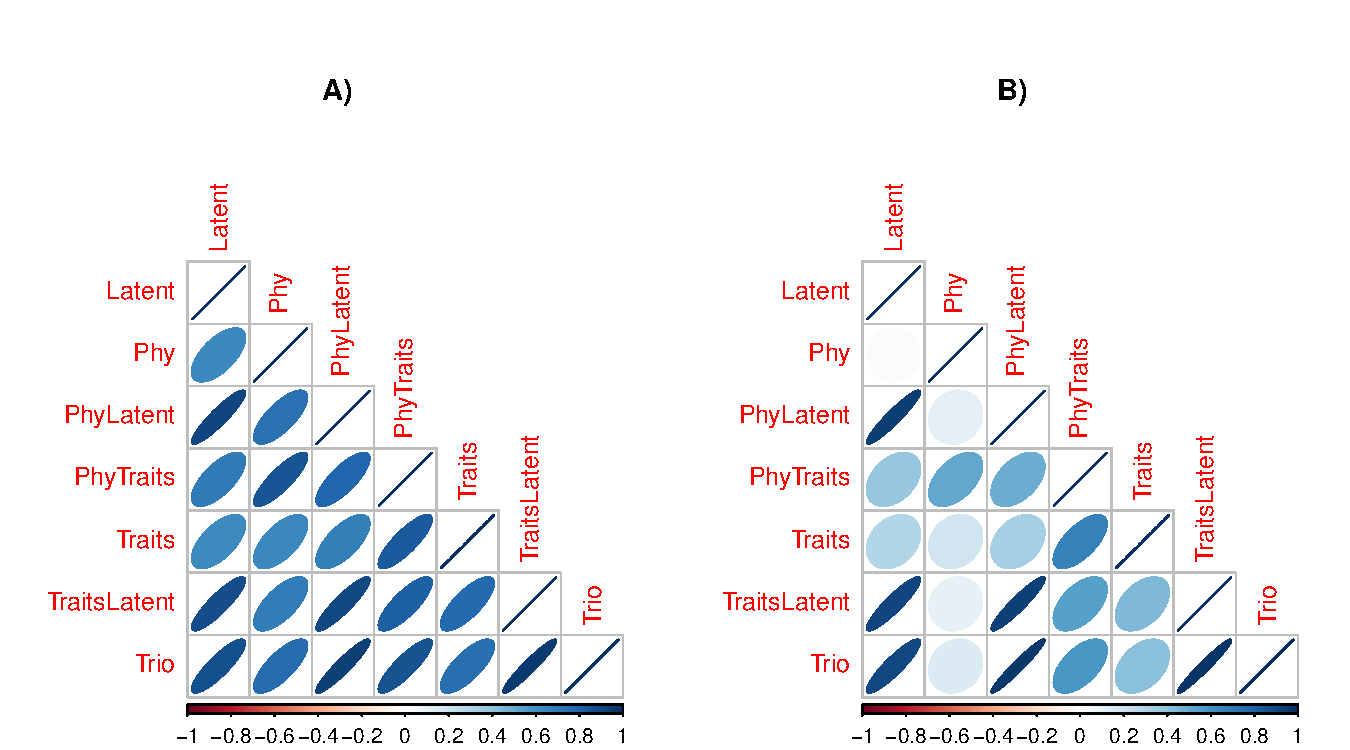
\includegraphics[width=\textwidth]{Fruglink/supplement/figs/fig3_nopoly.pdf}
    \caption[Link suitabilities across models when species without full phylogenetic information are excluded]{Pairwise Spearman's rank correlations of link suitabilities across models for all potential interaction (A), as well as only unobserved interactions (B), *after species without full phylogenetic information are excluded*. The latter set of links represents both true forbidden links, as well as other potential interactions not observed in our data-set.}
    \label{fig:FruglinkS5}
  \end{center}
\end{figure}


\paragraph*{Sensitivity to Class Imbalances}\mbox{}\\
In order to deal with the high degree of sparceness in our network, we trim the training set to enforce class balancing. In the maintext, we present the results of a 3:1 ratio unobserved:observed links. Here, show the methods is relatively insensitive to this exact proportion by repeating our analysis with alternative training ratios of 1:1 and 1:10.

\begin{figure}[H]
  \begin{center}
      \includegraphics[width=\textwidth]{Fruglink/supplement/figs/suitability_comp_unscaled.pdf}
    \caption[Scatterplot of relative suitability values of models trained under alternative prevalence values]{Scatterplot of relative suitability values of the same models trained under either a 1:3 ratio of present to absent interactions (y-axis) or a 1:1 ratio (x-axis); red dashed lines represent a 1:1 line. While the absolute value of suitability values tend to be reduced when the prevalence of true positives is reduced (most points fall below the 1:1 line), the relative rank of suitability values tends is very closely aligned (Spearman's $\rho = 0.964$ across all predictions).}
    \label{fig:FruglinkS6}
  \end{center}
\end{figure}


\begin{figure}[H]
  \begin{center}
      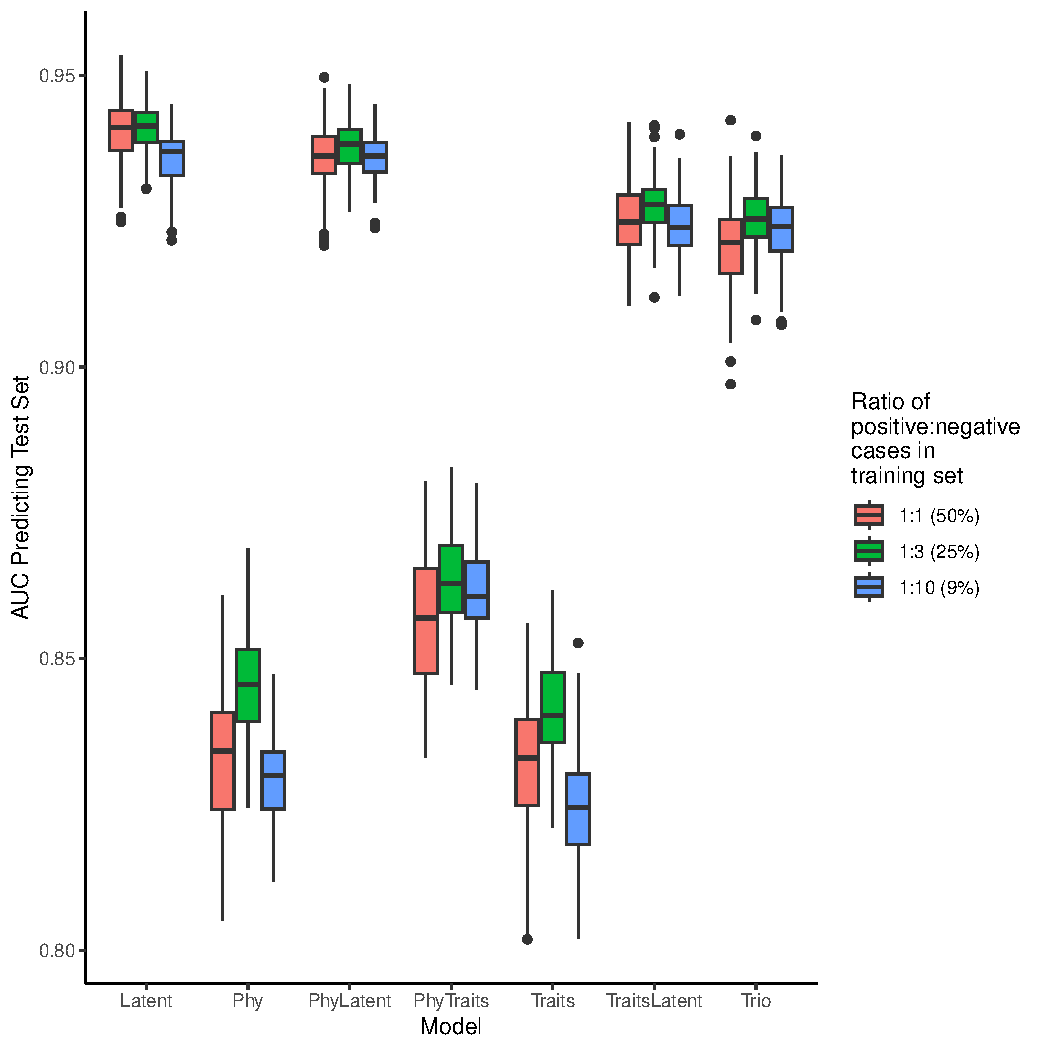
\includegraphics[width=\textwidth]{Fruglink/supplement/figs/AUC_Ratio.pdf}
    \caption[AUC of models trained under alternative prevalence values]{Box plots of AUC values for model predictions on a 20\% test set after being conditioned on training data with either 1:1, 1:3, or 1:10 ratios of presence to absence values. We see that while there is some variation in model performance according to training prevalence, the relative performance of each model is still qualitatively the same across the range of prevalence values. }
    \label{fig:FruglinkS7}
  \end{center}
\end{figure}


\begin{figure}[H]
  \begin{center}
      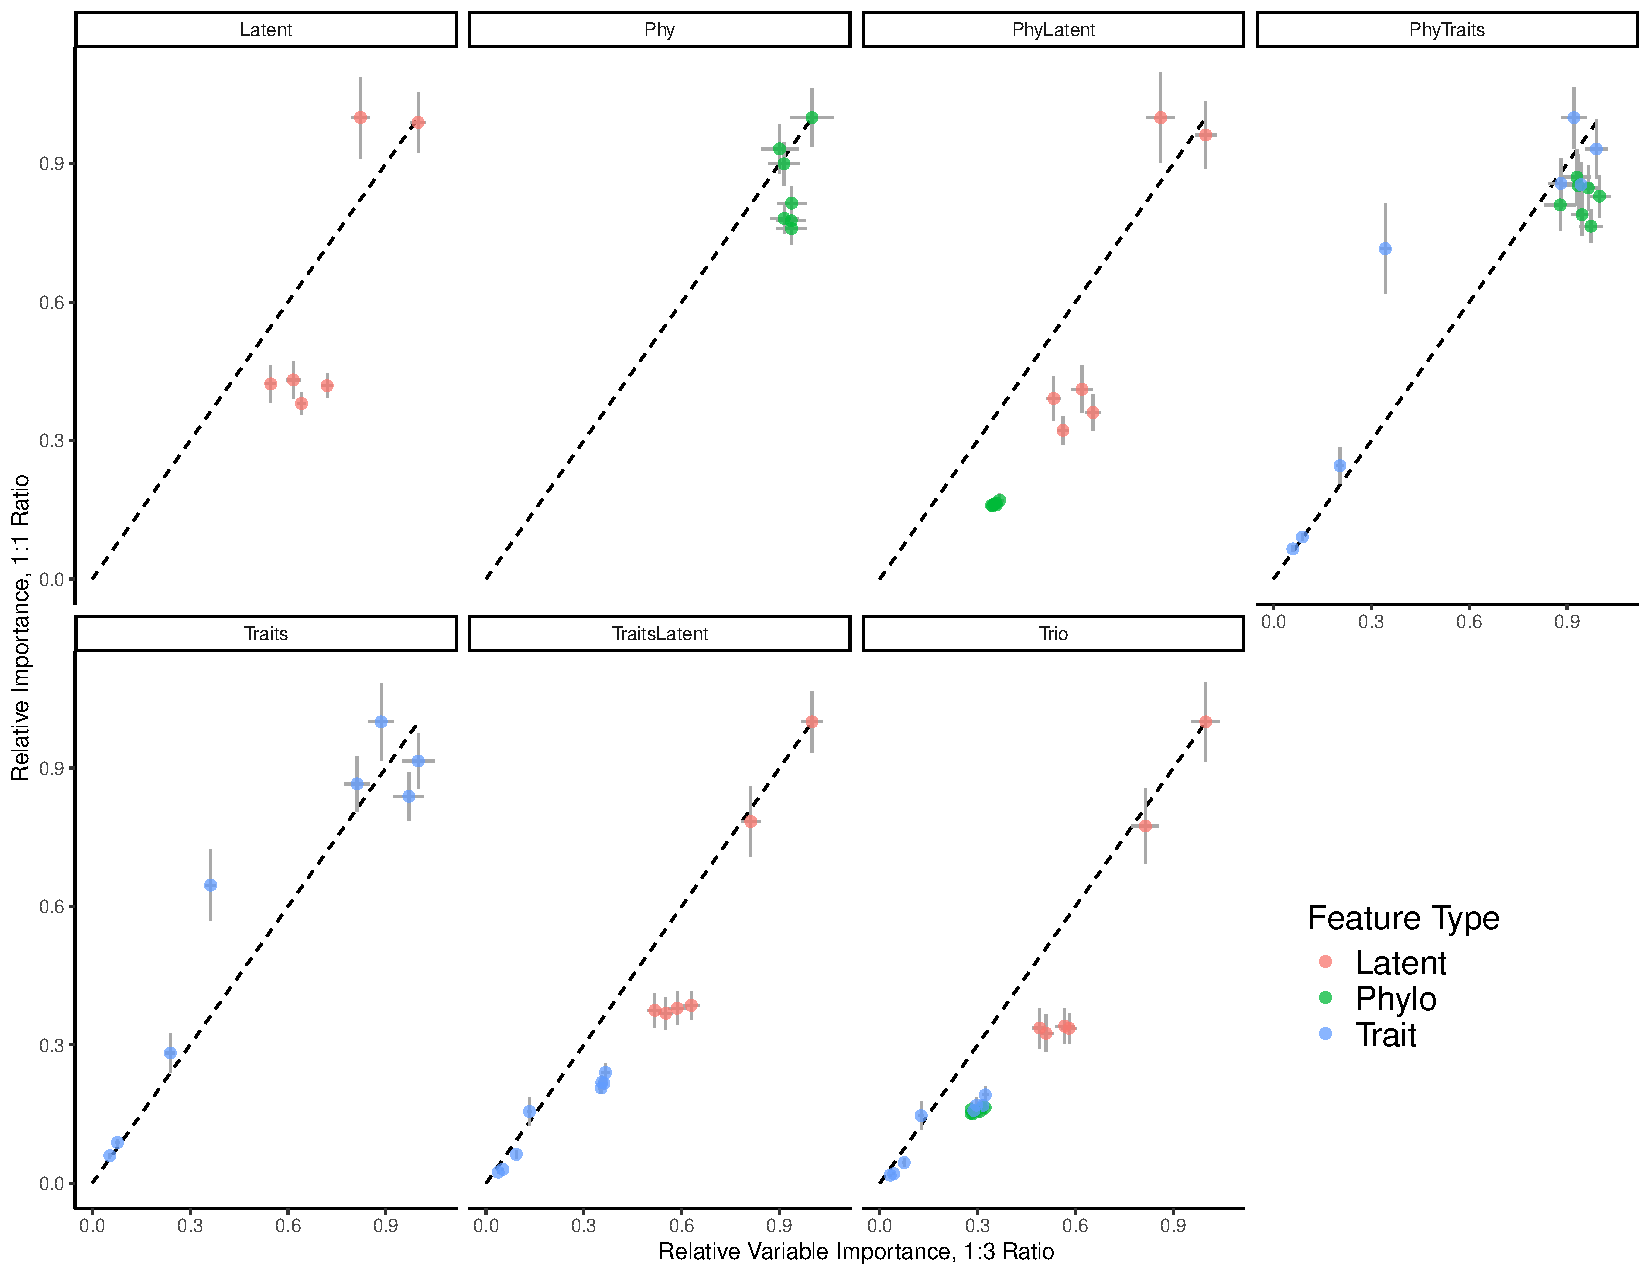
\includegraphics[width=\textwidth]{Fruglink/supplement/figs/Importance_by_Ratio.pdf}
    \caption[Variable importance of models trained under alternative prevalence values]{Variable importance between the same models trained on either a 1:1 ratio of present to absent interactions (y-axis) or a 1:3 ratio (x-axis). Dotted black lines represent a 1:1 line; points that fall on the line indicate that relative importance of that variable was unaffected by training prevalence. We see that the marjority of features fall very close to the 1:1 line, including the most important variables (top right of each inset plot).This indicates are models are realtively insensitive to training prevalence. }
    \label{fig:FruglinkS8}
  \end{center}
\end{figure}

\paragraph*{Sensitivity of Latent Traits to Incomplete Sampling}\mbox{}\\

Latent traits are derived from the observed network, which is an incomplete sample of some underlying "true" network that we're trying to predict. We might expect the ability of latent features to effectively predict links to be different across networks with different sample completeness. Here, we, attempt to characterize that sensitivity through a null model approach. 

The function below takes an arbitrary number of plants, frugivores, and "true" links between them and simulates a network based on those characteristics. Each frugivore and plant species is assigned an abundance value randomly drawn from a lognormal distribution. Links are randomly assigned across all potential interactions according to the abundance of both potential partners. Links between abundant species are more likely than links between rare species. While a simplistic, neutral process, this graph generation feature recapitulates long-tailed degree distributions and asymmetric specialization patterns frequently observed in empirical networks. 

Given this "true" observed network, we perform single-value decomposition to create latent features, extracting the first three axes of variation for all nodes as in the main text. From these features we create a euclidean distance matrix that represents the pairwise distances of each intraguild node combination in the three-dimensional space defined by these three latent trait axes. The result is $f \times f$ and $p \times p$  distance matrix, where `f` and `p` are the number of frugivores and plants, respectively. 

We then degrade this network, removing 50 links from the full set, again sampling non-randomly so that less abundant combinations of species are more likely to go unsampled. This serves to approximate an incomplete sampling process in an empirical system, where links between abundant partners are likely to be observed, but links between rare partners are more likely to be missed. We then repeat the process of single value decomposition and creation of an intriguild pairwise distance matrix. We then use spearman's rank correlations to compare the "true" distance matrix with that produced from the degraded network. If latent features are able to separate the ranks of most nodes even despite degradation, spearman's rank correlation should be high. However, if degrading the network severly alters node clustering, spearman's correlation should be low between the true and observed distance matrices. By repeating this process across a range of degradation values (each time comparing back to the "true" network), we can start to characterize the sensitivity of latent features to incomplete sampling. 

Below, we paramaterize the "true" model with 787 plant species, 242 frugivores, and 3643 "true" links, the same size as our empirically observed network. We repeat the process of degrading the network 50 times, and present average decreases in spearman's rank correlation. 


\begin{figure}[H]
  \begin{center}
      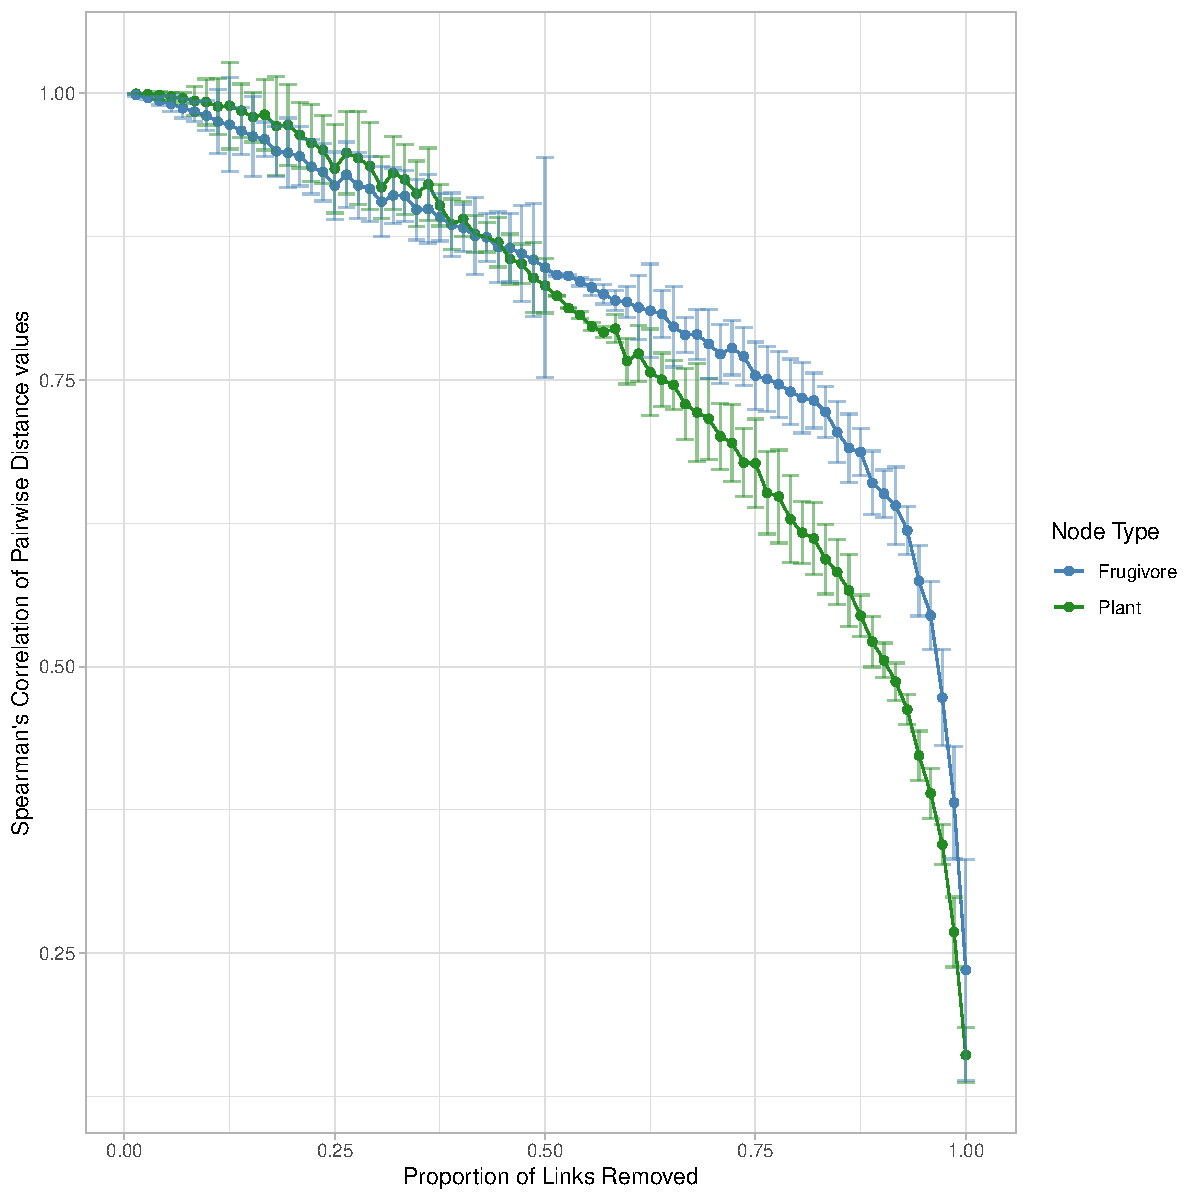
\includegraphics[width=\textwidth]{Fruglink/supplement/figs/decaysumplot.pdf}
    \caption[Plot of intraguild latent pairwise distance matrices derived from compared to the true network]{Plot of intraguild latent pairwise distance matrices derived from compared to the true network (spearman's rank correlation); lines represent mean values across 50 iterations, while error bars represent standard deviation. Correlation decreases as links are removed for both frugivore (blue) and plant (green) nodes, but generally decreases slowly until a high proportion of links are removed. Distance matrices exhibit $\rho>0.75$ for plant and frugivore species even after removing 64.5\% and 76.9\% of links, respectively. }
    \label{fig:FruglinkS9}
  \end{center}
\end{figure}


We also are interested in the ability of latent features to capture neutral processes given the aforementioned feature of incomplete sampling. Below, we simulate a number of "true" networks where attatchment is again only a function of species abundances drawn from a lognormal distribution. 

Next, we create a situation where empirical networks are generated using the generation process outlined above, and we again only observe a portion of the "true" links. We define a sampling rate, where we specify the number of observed links. 


We use singular value decomposition on this observed network, and use those features to inform a random forest model trained on the observed positive interactions and enough background points to create a 25\% prevalence. We evaluate this model through AUC on the held-out positive links as well as enough new background points to again achieve a 25\% prevalence on the test set. 

Below, we simulate this process across a variety of a) graph sizes, b) connectance values of the "true" graph, c) sampling completeness values, in order to characterize the potential of latent traits for prediction across this parameter space. This neutral case represents the *absolute simplest* case in which latent features may be useful. The only factors impacting species' probability of interacting are their respective abundances, while in real systems there may be many unmeasured factors impacting interaction structures which latent features may be able to detect. It is however a useful investigation into how latent features might change across this parameter space. The results of these simulations are found below. 


\begin{figure}[H]
  \begin{center}
      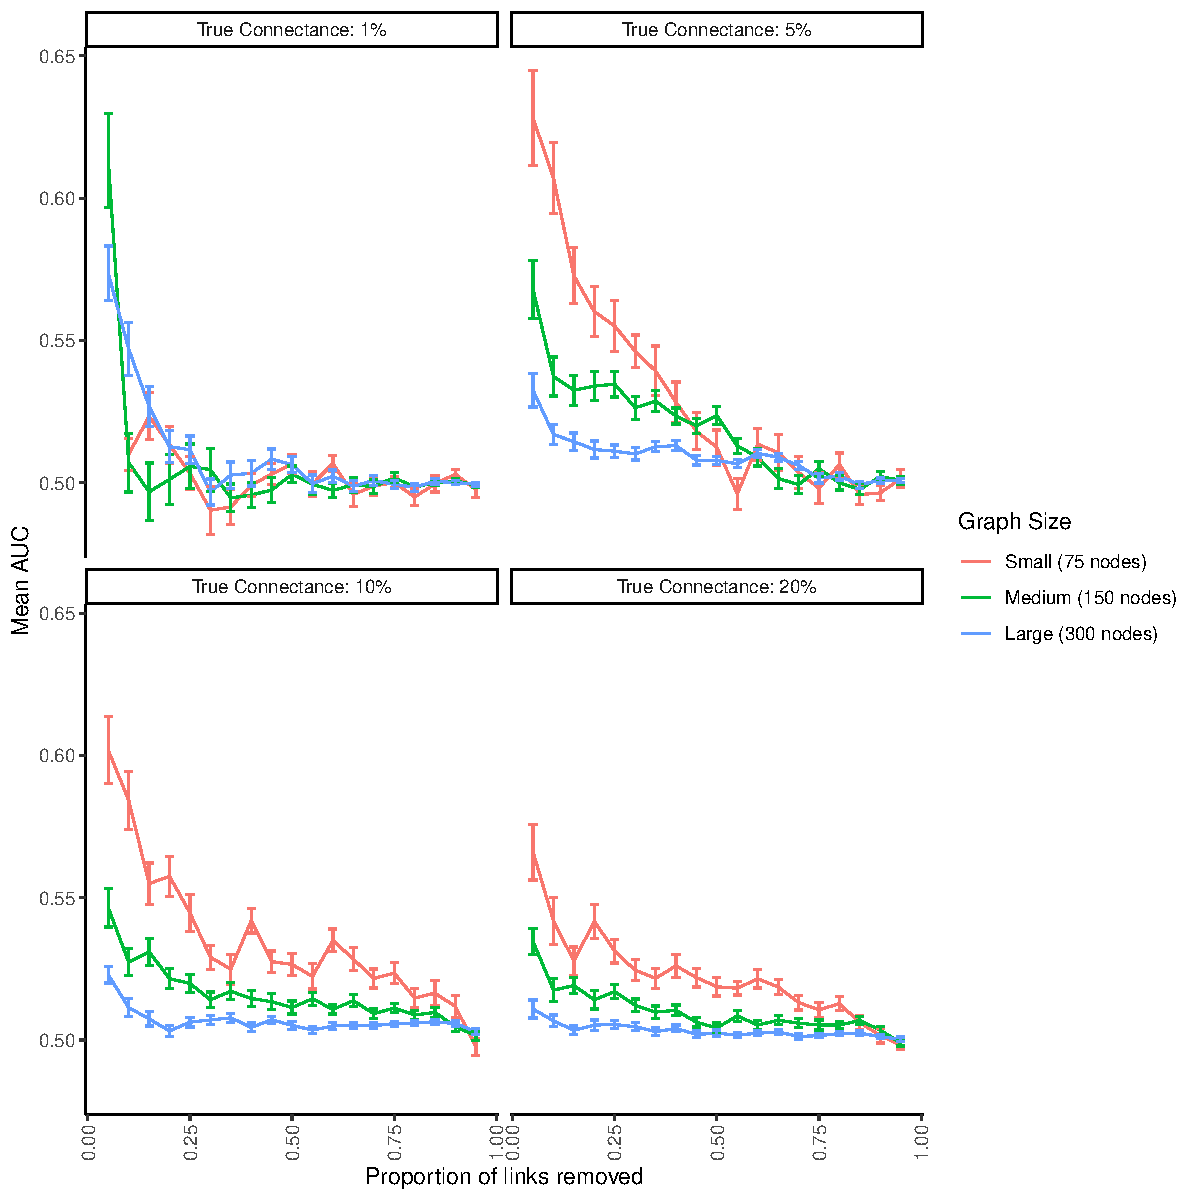
\includegraphics[width=\textwidth]{Fruglink/supplement/figs/nullsimulationResult.pdf}
    \caption[Plot of mean decrease in AUC performance as a function of the proportion of links removed from the observed set]{Plot of mean decrease in AUC performance as a function of the proportion of links removed from the observed set. Plot facets represent alternative connectance values of the true graph; color represent alternative graph sizes. Aside from the extreme sparse case (connectance = 1\%), latent features tended to perform best on the smallest graphs. Performance overall was highest on moderately sparse graphs (5\% connectance); across all connectance values and graph sizes, model performance decreases with greater sample degredation. }
    \label{fig:FruglinkS10}
  \end{center}
\end{figure}


In the main text version of this manuscript, while validating model performance (presented in Figure 1) we use a cross-validation approach suggested by Dr. Pedro Perez-Neto. In this approach, latent features are created for each test set independently, minimizing the chance of information leakage between test and train sets and thus facilitating comparisons of the predictive capacity of latent and non-latent features. When trying to impute missing links from a network in practice however, using the entirety of the network to create latent features is likely to improve performance. Below, we compare latent features created from these training subsets and those created from the full network. 


\begin{figure}[H]
  \begin{center}
      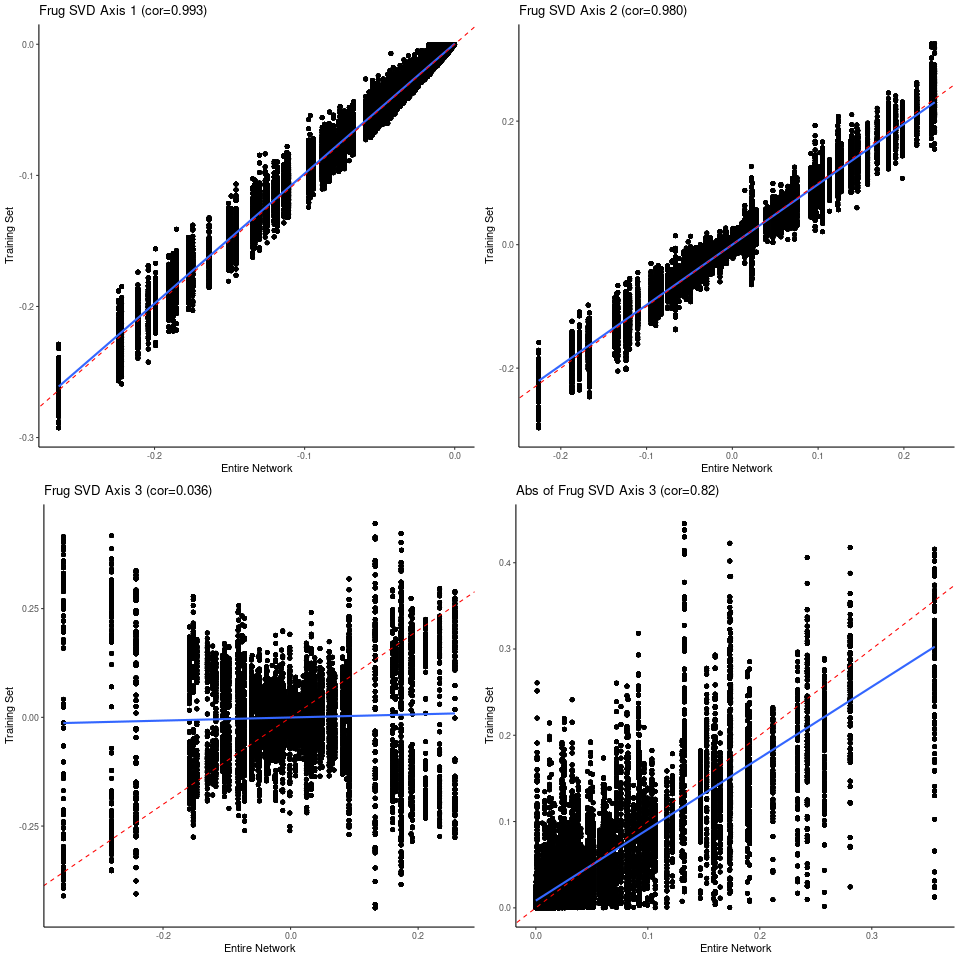
\includegraphics[width=\textwidth]{Fruglink/supplement/figs/Frugivore_cvComparison_small.png}
    \caption[SVD values for frugivores compared to those calculated from network subsets]{The first three SVD values for each frugivore species when calculated for from the entire network (x axis) and random 80\% training sets (y-axis). Red dashed lines are 1:1; blue solid lines show a best fit linear model. Pearson's correlation coefficients are presented in plot titles. Axes 1 and 2 are strongly related, even when a 20\% test set of interactions are witheld. While the exact relationship of axis 3 may be either positive or negative depending on the exact training values selected, the absolute values of the training subset are linearly related to the full networks. }
    \label{fig:FruglinkS11}
  \end{center}
\end{figure}

\begin{figure}[H]
  \begin{center}
      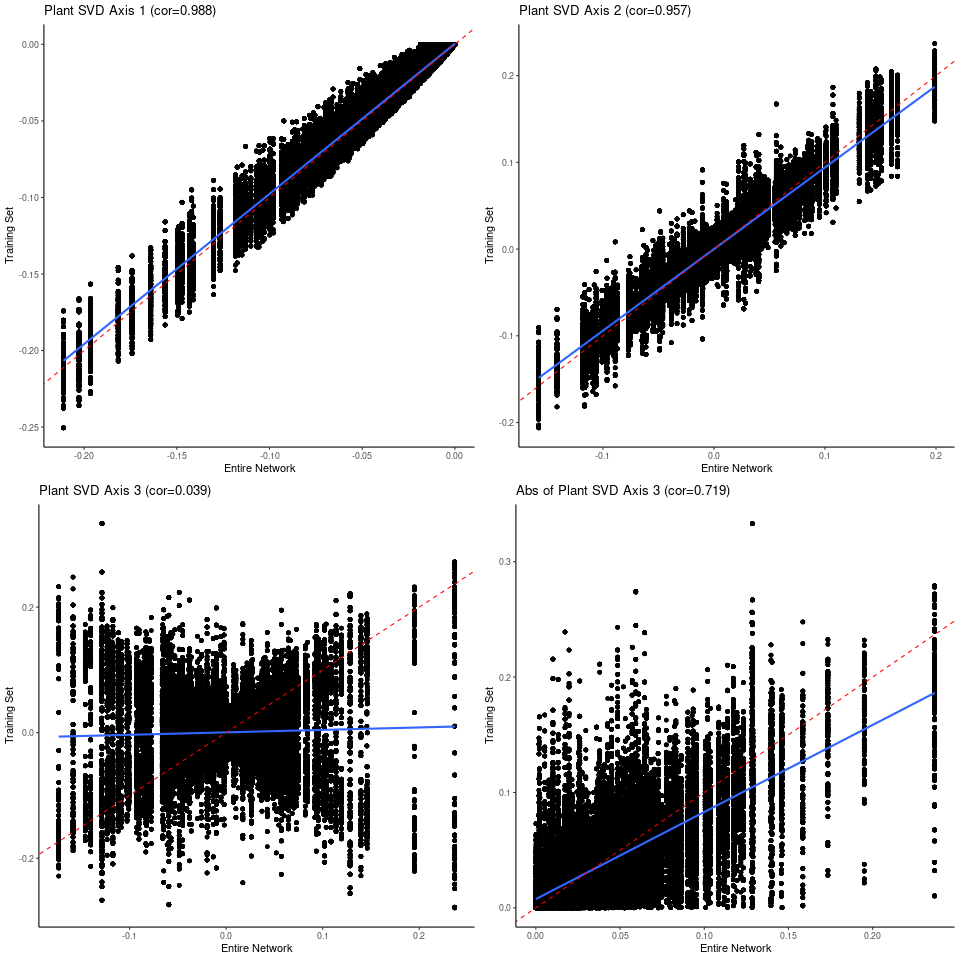
\includegraphics[width=\textwidth]{Fruglink/supplement/figs/Plant_cvComparison_Small.png}
    \caption[SVD values  for plants compared to those calculated from network subsets]{The first three SVD values for each plant species when calculated for from the entire network (x axis) and random 80\% training sets (y-axis). Red dashed lines are 1:1; blue solid lines show a best fit linear model. Pearson's correlation coefficients are presented in plot titles. Pearson's correlation coefficients are presented in plot titles. Similar to frugivores, axes 1 and 2 are strongly related, even when a 20\% test set of interactions are witheld. Again, while the exact relationship of axis 3 may be either positive or negative depending on the exact training values selected, the absolute values of the training subset are linearly related to the full networks. }
    \label{fig:FruglinkS12}
  \end{center}
\end{figure}



Below we repeat our main text analysis and illustrate predictive comparisons when latent features are created from the entire network, and then afterwards subsampled into test and training sets. In this way each individual model is still only trained on 80\% of observed interactions and corresponding background points, but the features associated with each interactions are created based on the entire network.

\begin{figure}[H]
  \begin{center}
      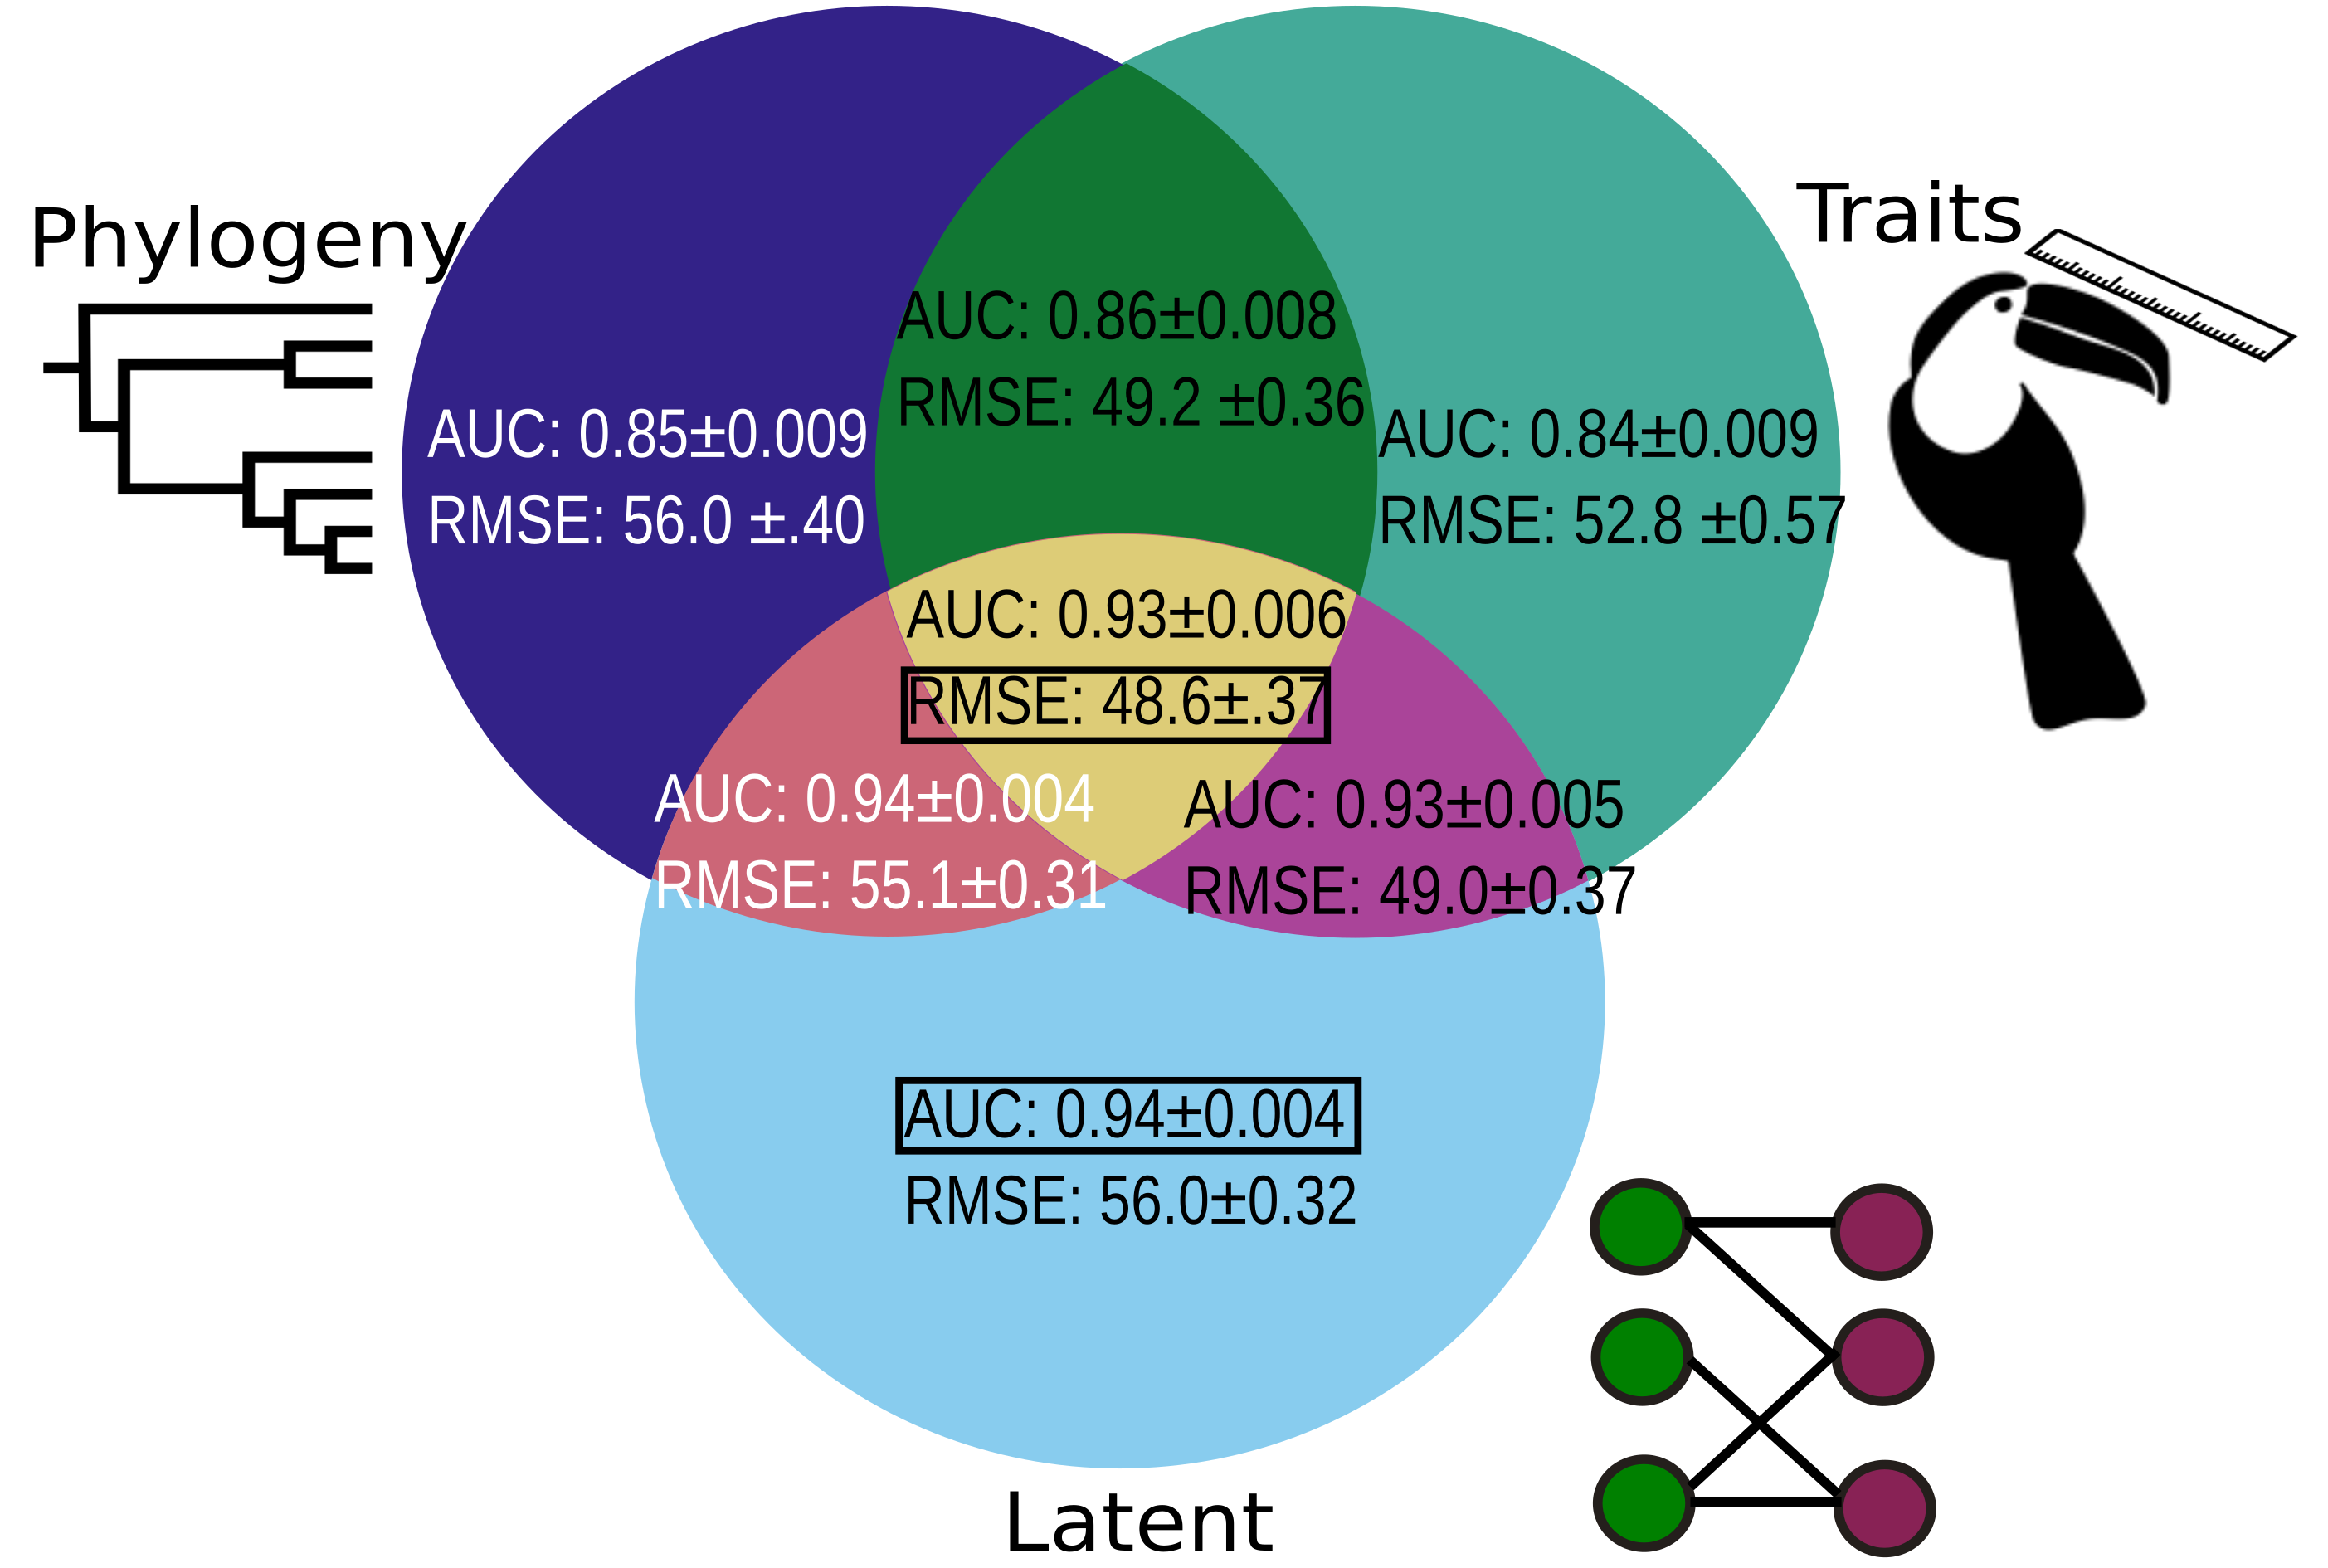
\includegraphics[width=\textwidth]{Fruglink/supplement/figs/NoCV_Fig1.png}
    \caption[ Model performance metrics when latent features are created from the entire network prior to dividing data into test and train sets.]{Model performance metrics when latent features are created from the entire network prior to dividing data into test and train sets. While slightly increasing the performance of latent features (potentially through some amount of information leakage between test and train sets), qualitative patterns as presented in the main text are still the same. }
    \label{fig:FruglinkS13}
  \end{center}
\end{figure}


\begin{figure}[H]
  \begin{center}
      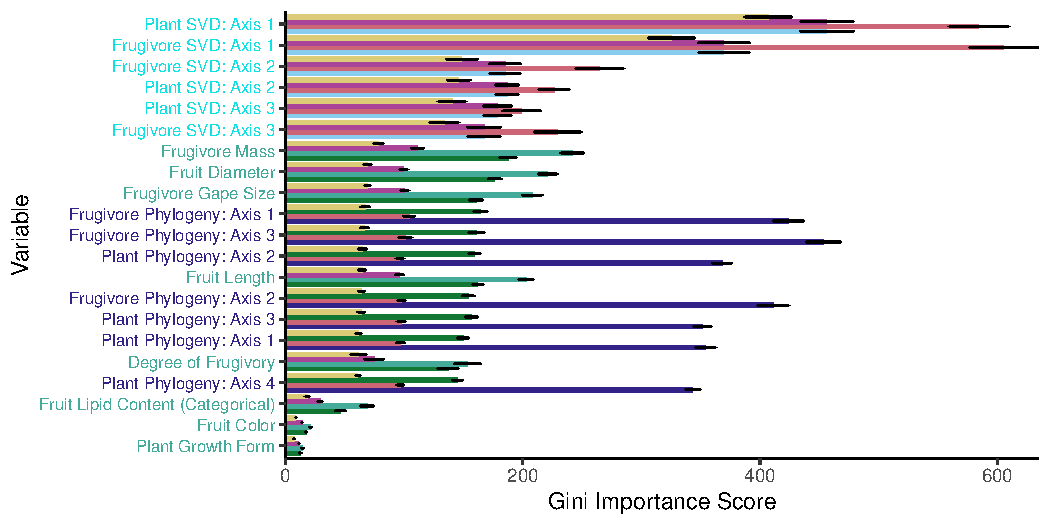
\includegraphics[width=\textwidth]{Fruglink/supplement/figs/VarImportance_ErrBars_Short_col2_withCV.pdf}
    \caption[Variable importance plots for models trained on 80\% training subsets, with latent features recalculated within each subset.]{Variable importance plots for models trained on 80\% training subsets, with latent features recalculated within each subset. The qualitative patterns are consistent with those observed when models are trained on the full interaction network without train–test splits (shown in Figure 2 of the main text). }
    \label{fig:FruglinkS14}
  \end{center}
\end{figure}

\begin{figure}[H]
  \begin{center}
      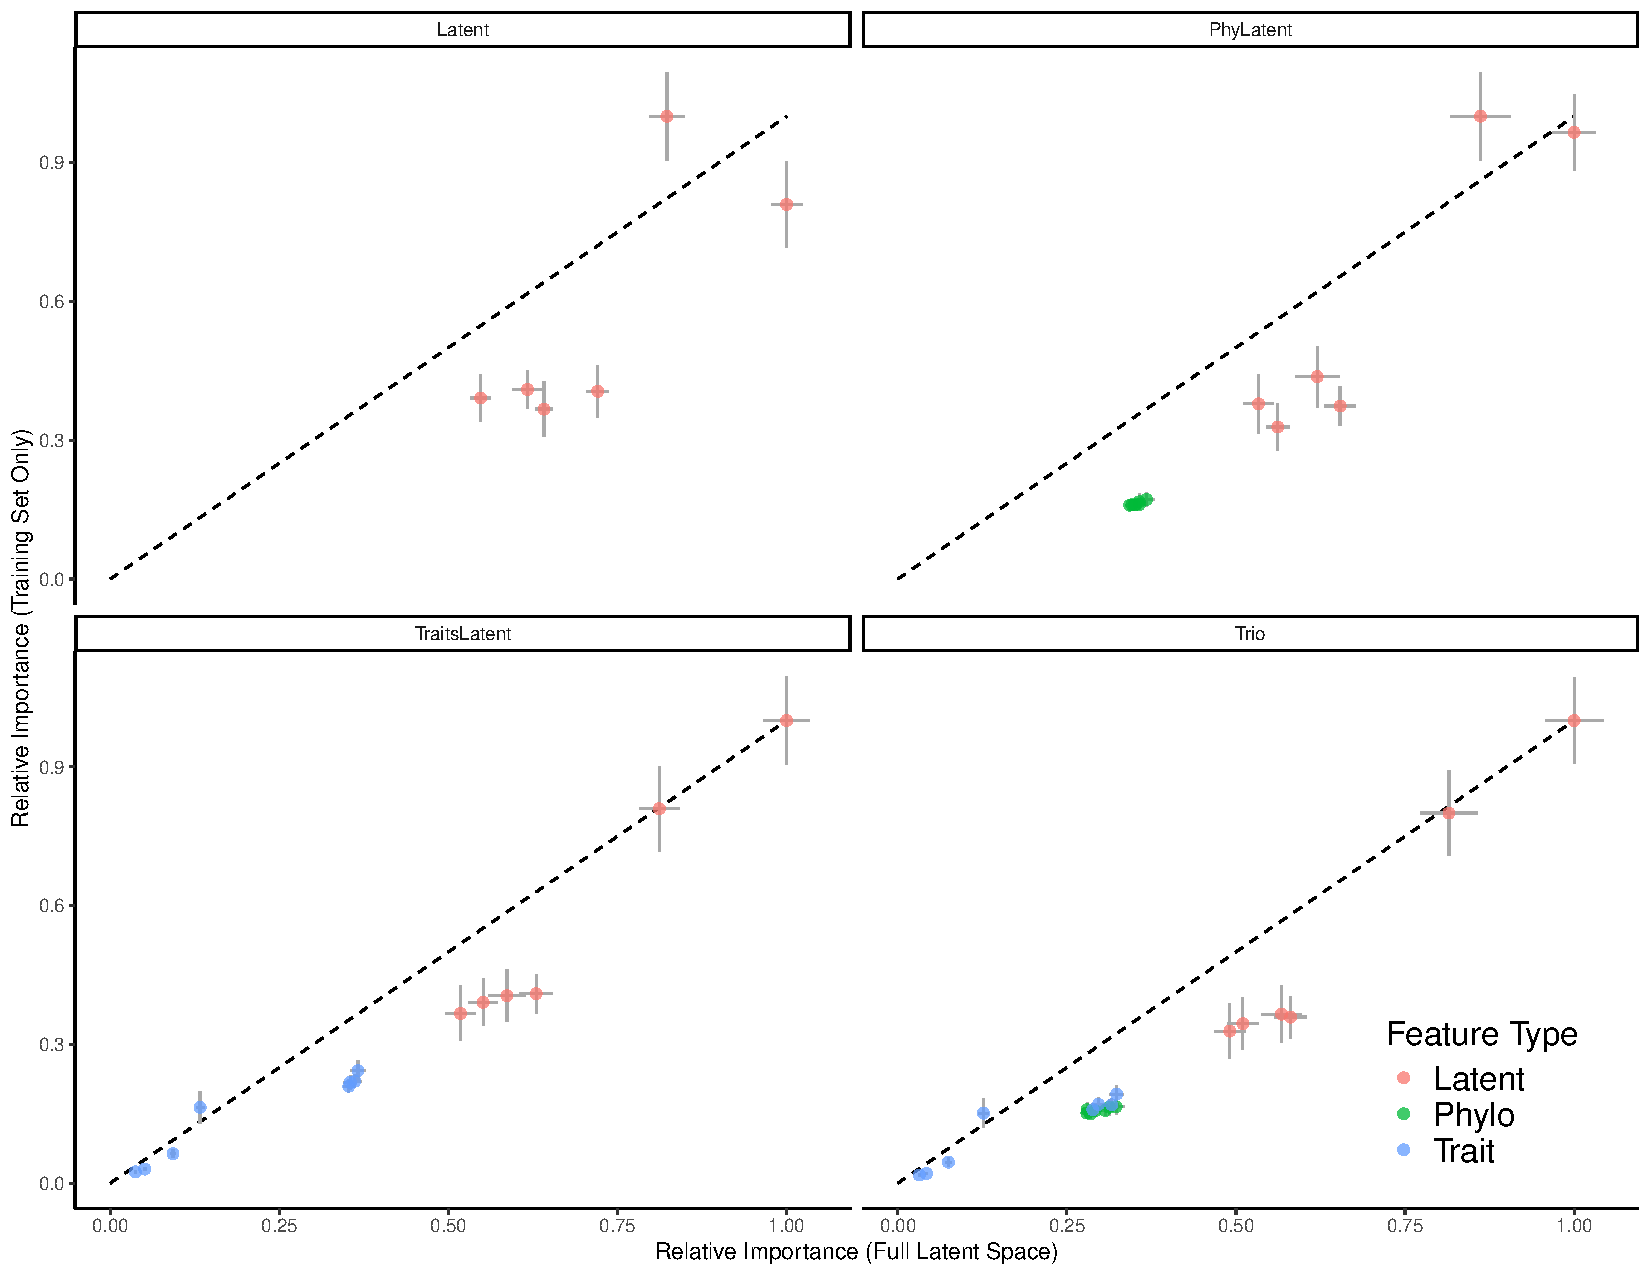
\includegraphics[width=\textwidth]{Fruglink/supplement/figs/Importance_comp_CV.pdf}
    \caption[Comparison of variable importance between the same models informed by latent features calculated from the entire network or only from 80\% training subsets]{Comparison of variable importance between the same models informed by latent features calculated from the entire network (x-axis) or only from 80\% training subsets (y-axis). Dotted black lines represent a 1:1 line; points that fall on the line indicate that relative importance of that variable was unaffected by the cross-validation procedure.We see that the majority of features fall relatively close to the 1:1 line, including the most important variables (top right of each inset plot). }
    \label{fig:FruglinkS15}
  \end{center}
\end{figure}